\section{Numerical calculation of dephasing rates}
\label{sec:numerical_rates}

This section validates the analytical predictions of the preceding section through full-system numerical simulations.

\subsection{Monte Carlo master equation simulation}
\label{subsec:monte_carlo}

The dynamics are simulated with the full Hamiltonian $H_{\mathrm{full}}(\delta\Phi)$ represented in a truncated oscillator (Fock) basis and evolved under the Lindblad master equation
\begin{align}
\dot{\rho}
&= -i\!\left[\,H_{\mathrm{full}}\big(\delta\Phi(t)\big),\ \rho\,\right]
+ \gamma_{b\downarrow}\,\mathcal{D}[b]\rho,
\label{eq:lindblad_full_ch8}
\end{align}
where $\mathcal{D}[b]\rho=b\rho b^\dagger-\tfrac{1}{2}\{b^\dagger b,\rho\}$.
\paragraph{Generation of $1/f$ noise.} Flux noise is incorporated through stochastic trajectories $\delta\Phi(t)$ whose spectrum
follows a $1/f$ power spectral density. For each trajectory, Eq.~\eqref{eq:lindblad_full_ch8}
is integrated to obtain $\rho(t)$, and all reported curves are computed from ensemble
averages of the corresponding observables. The noise realizations $\delta\Phi(t)$ are
generated using the frequency-domain synthesis method of Ref.~\cite{timmer1995generatingcolornoise}:
Fourier components are assigned random phases and Gaussian-distributed amplitudes with
variances proportional to the target $1/f$ spectrum, followed by an inverse Fourier
transform to obtain $\delta\Phi(t)$ in the time domain. Fig.~\ref{fig:psd_ch8} shows the
resulting power spectral densities for 100 representative trajectories. This ensemble size
is sufficient for the quantities of interest to converge, as indicated by the small error
bars in Fig.~\ref{fig:total_rate}(a) and Fig.~\ref{fig:relaxation_excitation_plot}(b).

\begin{figure}[H]
    \centering
    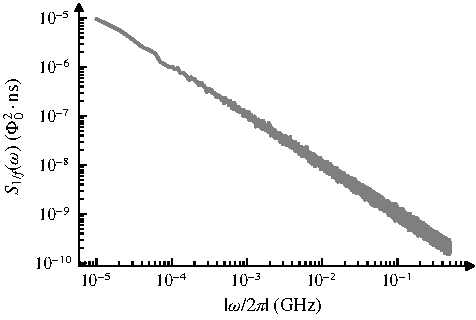
\includegraphics[width=\linewidth]{chapter8/figures/noise_spectrum_plot.pdf}
    \caption{Power spectral density of $\delta\Phi(t)$ for 100 representative $1/f$ noise
    trajectories generated with the cutoffs specified below.}
    \label{fig:psd_ch8}
\end{figure}

The total simulated evolution time is $T\sim 10~\mu\mathrm{s}$, and the infrared cutoff
is set to $\omega_{\mathrm{IR}}/2\pi=10~\mathrm{kHz}$ (equivalently
$f_{\min}=10^{-5}\,\mathrm{GHz}$). This choice satisfies $f_{\min}\ll 1/T \approx 100~\mathrm{kHz}$,
capturing the relevant slow-noise dynamics within the simulated window while avoiding the
infrared divergence of an ideal $1/f$ spectrum. The ultraviolet cutoff is set to
$f_{\max}=1~\mathrm{GHz}$; the extracted dephasing rates are insensitive to further
increases of $f_{\max}$.

\paragraph{Extraction of dephasing time.} The states with enhanced dephasing discussed in the preceding chapters are proxies for the corresponding Floquet states, as shown in Sec.~\ref{sec:floquet}.
In the numerics, Floquet modes are labeled by their correspondence to bare states as
described in Appendix~\ref{app:numerics}. The two Floquet states used for the cavity
dephasing analysis
are denoted $\ket{\phi_{g,0}(t)}$ and $\ket{\phi_{g,1}(t)}$.

Relaxation and dephasing are extracted from dynamics evolving from two initial states. Relaxation is
characterized by preparing
\[
\rho(0)=\ket{\phi_{g,1}(0)}\!\bra{\phi_{g,1}(0)}
\]
and monitoring the return toward \(\ket{\phi_{g,0}(t)}\). Dephasing is characterized by preparing the equal superposition
\[
\rho(0)=\ket{+}\!\bra{+},
\qquad
\ket{+}=\frac{1}{\sqrt{2}}\Big(\ket{\phi_{g,0}(0)}+\ket{\phi_{g,1}(0)}\Big),
\]
and tracking the decay of the corresponding coherence. The relevant quantities are
\[
\mathrm{Tr}\!\left[\rho(t)\,P_{g,0}(t)\right]
\quad \text{and} \quad
\mathrm{Tr}\!\left[\rho(t)\,X(t)\right],
\]
where
\[
P_{g,0}(t)=\ket{\phi_{g,0}(t)}\!\bra{\phi_{g,0}(t)},
X(t)=\ket{\phi_{g,1}(t)}\!\bra{\phi_{g,0}(t)}+\mathrm{H.c.}
\]


Relaxation and dephasing times are obtained by fitting ensemble-averaged signals.
Specifically, $T_1$ is extracted from the rise of the ground-state population by fitting
$\mathrm{Tr}\!\left[P_{g,0}(t)\,\overline{\rho}(t)\right]$ to $1-e^{-t/T_1}$, where
$\overline{\rho}(t)$ denotes the ensemble-averaged density matrix over different flux noise trajectories. The coherence time $T_2$
is extracted from the decay of the superposition signal by fitting
$\mathrm{Tr}\!\left[P_{+}(t)\,\overline{\rho}(t)\right]$ to $e^{-t/T_2}$ (with the appropriate
normalization convention for the plotted data). The pure dephasing time then follows from
\begin{align}
\frac{1}{T_\phi}=\frac{1}{T_2}-\frac{1}{2T_1},
\end{align}
and we report the total dephasing rate as $\Gamma_{\phi,\mathrm{total}}=1/T_\phi$.

\subsection{Benchmarking individual dephasing channels}
\label{subsec:check_individual}

This subsection benchmarks the analytical dephasing rates in Eq.~\eqref{eq:Gamma_phi_total_unselective} against numerical simulations. The numerical reference rate for
\(\gamma_{b\uparrow}^{\mathrm{un}}+\gamma_{c\phi}^{\mathrm{un}}\) is extracted using the Monte Carlo procedure of Sec.~\ref{subsec:monte_carlo}, with the flux-noise drive set to \(\delta\Phi(t)=0\).

In the large-detuning regime, the reference rate is well captured by the analytical approximation in Fig.~\ref{fig:relaxation_excitation_plot}(a):
\begin{align}
&\gamma_{b\uparrow}^{\mathrm{un}}+\gamma_{c\phi}^{\mathrm{un}}\\
&=
\frac{\gamma_{b\downarrow}}{16}\left(\frac{\Delta_{bd}}{K}\right)^2
\left(1-\frac{2\Delta_{bd}}{K}\right)
+\frac{\gamma_{b\downarrow}}{2}\left(\frac{g}{\Delta_{bc}}\right)^4\frac{K}{\Delta_{bd}} .
\label{eq:gamma_unselective_approx}
\end{align}

In this limit, dephasing is dominated by photon-shot noise from heating, i.e., \(\gamma_{b\uparrow}^{\mathrm{un}}\), while \(\gamma_{c\phi}^{\mathrm{un}}\) is parametrically suppressed at large detuning, consistent with Eq.~\eqref{eq:gamma_unselective_approx}.

As the detuning decreases, the numerical and analytical results deviate because Eq.~\eqref{eq:gamma_unselective_approx} assumes \(|\Delta_{bd}/\chi|\gg 1\) (here \(\chi/2\pi \simeq -2\,\mathrm{MHz}\)). In this regime, the total dephasing rate increases and \(\gamma_{c\phi}^{\mathrm{un}}\) becomes the dominant contribution.

Finally, the flux-noise-induced depolarization rate is benchmarked numerically against
\begin{equation}
\gamma_{b\uparrow}^{1/f,\mathrm{un}}=
\left(\frac{\partial\omega_b}{\partial\Phi}\right)^2\frac{S_0^2}{4K}.
\end{equation}
The simulation is initialized in the Floquet ground state \(|\phi_{g0}(0)\rangle\), and the excitation rate is extracted by fitting the average overlap
\(\mathrm{Tr}\!\left[\rho\,|\phi_{g0}(0)\rangle\langle\phi_{g0}(0)|\right]\) to \(\frac{1}{2}\!\left(1-e^{-2\gamma_{b\uparrow}^{1/f,\mathrm{un}} t}\right)\).
Sweeping the noise amplitude \(S_0\) yields a quadratic scaling, and the numerical results follow the analytical prediction (black dashed line) closely [Fig.~\ref{fig:relaxation_excitation_plot}(b)]. The small error bars in the figure indicate statistical convergence for the chosen ensemble size ($N=100$ trajectories).

\begin{figure}[H]
    \centering
    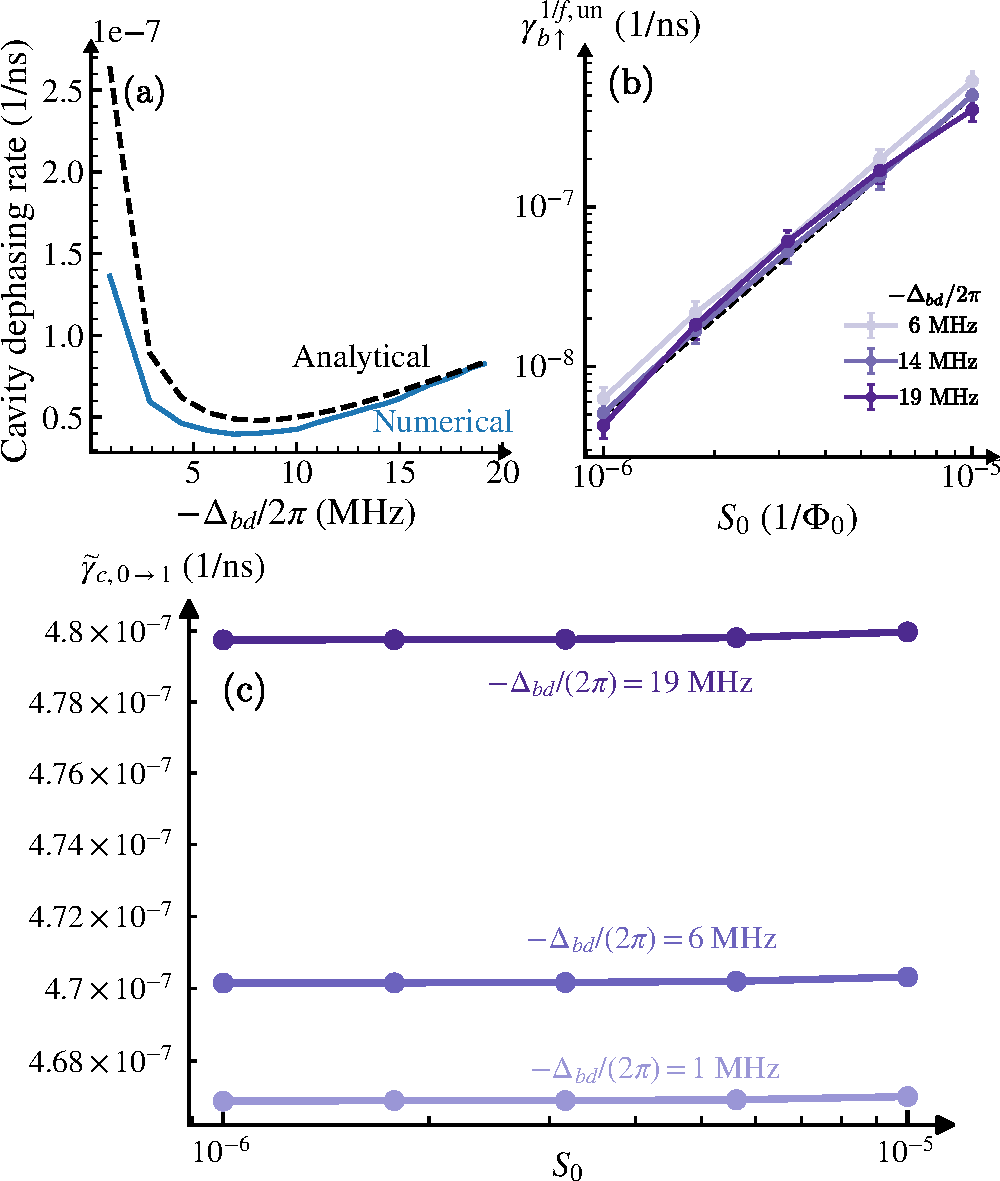
\includegraphics[width=\linewidth]{chapter8/figures/relaxation_excitation_plot.pdf}
    \caption{Numerical validation of rates in the unselective regime.
(a) Reference dephasing rate \(\gamma_{b\uparrow}^{\mathrm{un}}+\gamma_{c\phi}^{\mathrm{un}}\) extracted from Monte Carlo simulations with \(\delta\Phi(t)=0\), compared with the analytical approximation in Eq.~\eqref{eq:gamma_unselective_approx}.
(b) Flux-noise-induced depolarization rate \(\gamma_{b\uparrow}^{1/f,\mathrm{un}}\) versus noise amplitude \(S_0\). The quadratic scaling in \(S_0\) and agreement with \(\gamma_{b\uparrow}^{1/f,\mathrm{un}}=\left(\frac{\partial\omega_b}{\partial\Phi}\right)^2\frac{S_0^2}{4K}\) (black dashed line) are observed.
(c) Cavity decay rate with sweet-spot drive.}
    \label{fig:relaxation_excitation_plot}
\end{figure}

This subsection also shows that the cavity decay rate is only weakly affected by the drive. For the parameters used to generate Fig.~\ref{fig:total_rate}, the undriven decay rate is \(4.75\times10^{-7}\,\mathrm{ns}^{-1}\). Under drive, the decay rate remains nearly unchanged, as shown in Fig.~\ref{fig:relaxation_excitation_plot}(c). Under the analytical approximation in Eq.~\eqref{eq:Gamma_phi_total_unselective}, each contribution agrees well with the numerical simulations.

\subsection{Total dephasing rate}
\label{subsec:total_dephasing_numerical}

Full-system simulations are used to extract the cavity dephasing rate under drive; the
numerical procedure and fitting protocol are summarized in Sec.~\ref{subsec:monte_carlo}.
The noise amplitude $S_0$ and the detuning $\Delta_{bd}$ are sampled over the parameter
range of interest. For each $\Delta_{bd}$, the drive amplitude is chosen to satisfy the
sweet-spot condition, and the corresponding total dephasing rate
$\Gamma_{\phi,\mathrm{total}}$ is extracted.

Fig.~\ref{fig:total_rate}(a) summarizes the results. For $S_0=10^{-5}/\Phi_0$, the
drive-induced contribution $\gamma_{b\uparrow}^{1/f,\mathrm{un}}$ dominates
$\Gamma_{\phi,\mathrm{total}}$ over the scanned detuning range. At large detuning,
$\lvert\Delta_{bd}\rvert> \lvert\chi\rvert\simeq 2~\mathrm{MHz}$, the total rate is well described by $\gamma_{b\uparrow}^{1/f,\mathrm{un}}$, which is independent of the detuning. At smaller detuning, i.e.\
$-\Delta_{bd}/2\pi=1~\mathrm{MHz}<\lvert\chi/2\pi\rvert$, the rate
increases as the dynamics enters the selective regime, consistent with the
$1/\lvert\Delta_{bd}\rvert$ scaling.

For smaller noise amplitude, e.g.\ $S_0=10^{-6}/\Phi_0$, the $S_0$-independent drive-induced contributions
$\gamma_{b\uparrow}^{\mathrm{un}}$ and $\gamma_{c\phi}^{\mathrm{un}}$ dominate
$\Gamma_{\phi,\mathrm{total}}$. At large detuning ($-\Delta_{bd}/2\pi=19~\mathrm{MHz}$),
$\gamma_{b\uparrow}^{\mathrm{un}}\propto(\Delta_{bd}/K)^2$ dominates while
$\gamma_{c\phi}^{\mathrm{un}}\sim K/\Delta_{bd}$ is suppressed; the opposite hierarchy
holds at small detuning ($-\Delta_{bd}/2\pi=1~\mathrm{MHz}$). Consequently,
$-\Delta_{bd}/2\pi=6~\mathrm{MHz}$ yields the minimal $\Gamma_{\phi,\mathrm{total}}$
within the scanned range. In the undriven case, the dephasing time is
$\sim 0.1$--$1~\mathrm{ms}$ as $S_0$ varies from $10^{-5}/\Phi_0$ to $10^{-6}/\Phi_0$. With $\Delta_{bd}/2\pi\simeq -6~\mathrm{MHz}$ and
sweet-spot driving, the dephasing time improves by up to $\sim 20\times$ across the
considered $S_0$ range, confirming the overall dephasing enhancement.

\begin{figure}[H]
    \centering
    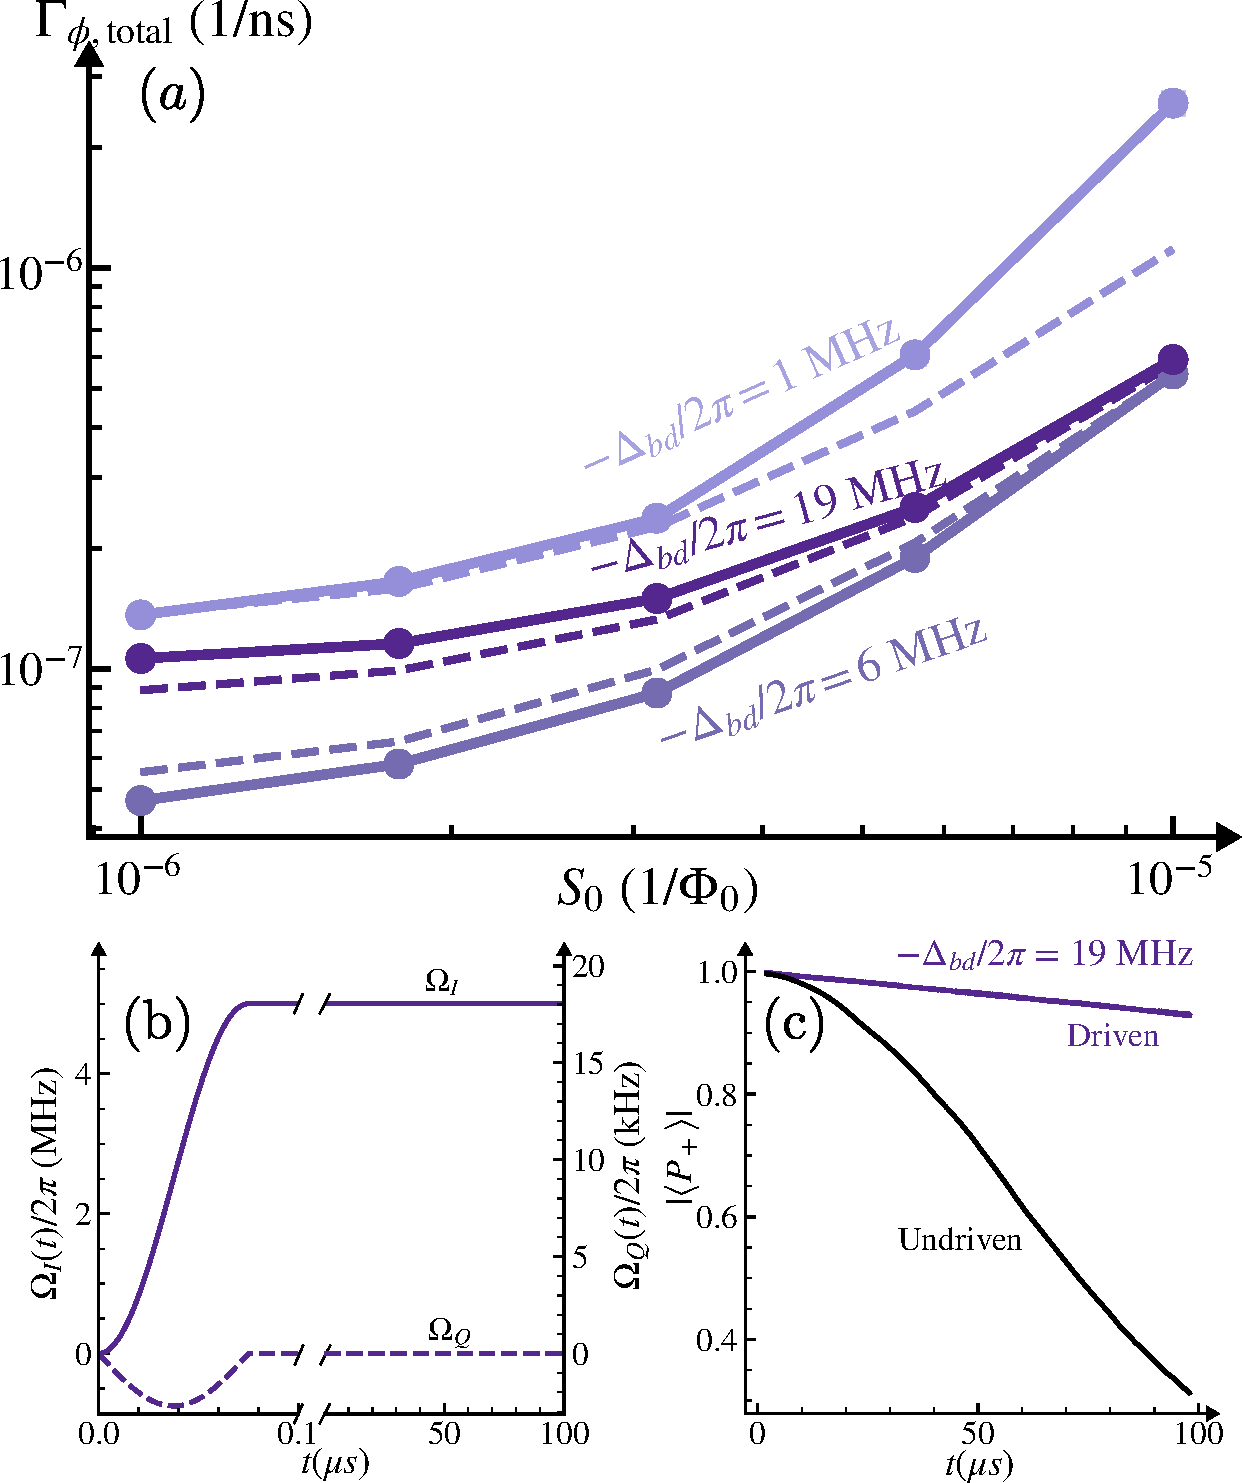
\includegraphics[width=\linewidth]{chapter8/figures/total_rate.pdf}
    \caption{Numerical evaluation and time-domain validation of the total cavity dephasing
    rate under sweet-spot driving. (a) Total dephasing rate $\Gamma_{\phi,\mathrm{total}}$
    extracted from full-system simulations as a function of detuning $\Delta_{bd}$, with
    the drive amplitude chosen at each detuning to satisfy the sweet-spot condition.
    $S_0$ denotes the amplitude of $1/f$ flux noise. (b) DRAG-style adiabatic ramp pulse.
    (c) Time-domain decay of
$P_X(t)=\mathrm{Tr}\!\left[\rho(t)\,X(t)\right]$, with
$X(t)=\ket{\phi_{g,1}(t)}\!\bra{\phi_{g,0}(t)}+\mathrm{H.c.}$.
The time-dependent Floquet states are labeled by their bare-state correspondence.
The driven system exhibits a cavity dephasing time of $\sim 2~\mathrm{ms}$,
compared to $\sim 100~\mu\mathrm{s}$ in the undriven case.}
    \label{fig:total_rate}
\end{figure}

To visualize the dephasing enhancement directly, we perform time-domain simulations that
include relaxation and stochastic flux noise with $S_0=10^{-5}/\Phi_0$. The initial state is
$\ket{\psi_0}=\tfrac{1}{\sqrt{2}}\big(\ket{g,0}+\ket{g,1}\big)$. With drive, the state is
adiabatically mapped onto the target Floquet states using a shaped pulse
$2\Omega_0(t)\cos\!\big(\omega t+\phi(t)\big)$. In the rotating frame this yields the
$I$ and $Q$ quadratures
\begin{align}
\Omega_I(t) = \Omega(t)\cos\phi(t), \qquad
\Omega_Q(t) = \Omega(t)\sin\phi(t).
\end{align}
We implement a DRAG correction,
$\Omega_Q(t) = -\dot{\Omega}_I(t)/\Delta_{bd}$, which accelerates the adiabatic transfer
relative to $\Omega_I(t)$-only ramps (see Sec.~\ref{sec:adiabatic_transition}). A pulse ramp
with $\tau=75~\mathrm{ns}$ is shown in Fig.~\ref{fig:total_rate}(b).

The dephasing is quantified by the coherence operator
\begin{align}
X(t) &= \ket{\phi_{g,1}(t)}\!\bra{\phi_{g,0}(t)} + \mathrm{H.c.}, \\
P_X(t) &= \mathrm{Tr}\!\left[\rho(t)\,X(t)\right],
\end{align}
where $\ket{\phi_{g,1}(t)}$ and $\ket{\phi_{g,0}(t)}$ are adiabatically mapped from the bare states.
Without drive, \(1/f\) noise produces sub-Gaussian free-induction decay. At the driven sweet spot, the dominant residual channel is Markovian, arising from FTT depolarization, and yields the exponential decay observed in Fig.~\ref{fig:total_rate}(c). The dephasing time \(T_2\) is extracted from an exponential fit to \(P_X(t)\). Under sweet-spot driving, the dephasing time reaches \(\sim 2~\mathrm{ms}\), compared with \(\sim 100~\mu\mathrm{s}\) in the undriven case.
